\subsection{Dynamic Time Warping}\label{sub:DTW}
\begin{figure}[htb]
	\centering
	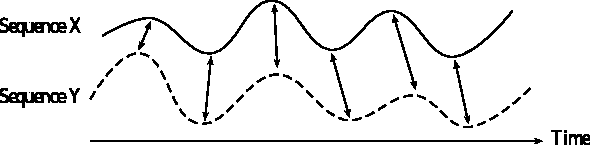
\includegraphics{dtw.pdf}
	\caption{Χρονική ευθυγράμμιση δύο χρονοσειρών $X, Y$}
\end{figure}
\begin{figure}
	\centering
	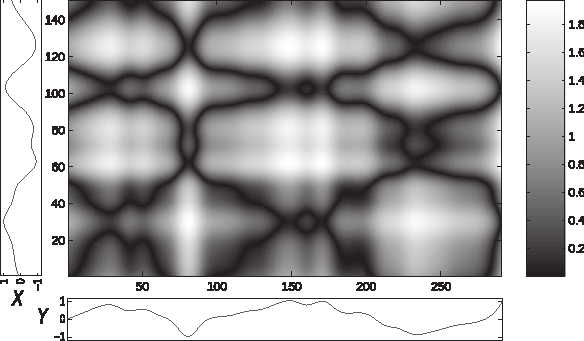
\includegraphics{dtw_cost.pdf}
	\caption{Ενδεικτικός πίνακας κόστους DTW για δύο χρονοσειρές $X, Y$}
\end{figure}
Το Dynamic Time Warping (DTW) είναι ένας αλγόριθμός που μετράει την ομοιότητα
μεταξύ δύο χρονοσειρών οι οποίες μπορεί να διαφέρουν στην ταχύτητά τους.
Ουσιαστικά, δοσμένων δύο χρονοσειρών $\vec x, \vec y$ η απόσταση κατά DTW
δίνεται από τον αναδρομικό τύπο
$$
D^2_{DTW} \left(\vec x, \vec y\right) = D^2 \left(First \left(\vec x\right), First \left(\vec y\right)\right) + \min \begin{cases} D^2_{DTW} \left(\vec x, Rest \left(\vec y\right)\right) \\
 D^2_{DTW} \left(Rest \left(\vec x\right),\vec y\right) \\
 D^2_{DTW} \left(Rest \left(\vec x\right), Rest \left(\vec y\right)\right) \end{cases}
$$
όπου οι τελεστές $First \left( \cdot\right), Rest \left( \cdot\right)$
επιστρέφουν το πρώτο στοιχείο μιας χρονοσειράς και το υπόλοιπο της χρονοσειράς
(χωρίς το πρώτο στοιχείο) αντίστοιχα.
Η εύρεση της ελάχιστης DTW απόστασης μπορεί να παρομοιαστεί με το κλασσικό
πρόβλημα δυναμικού προγραμματισμού Longest Common Subsequence (LCS).
Περαιτέρω τεχνικές λεπτομέρειες διαφεύγουν της σκοπιμότητας αυτής της αναφοράς,
και για αυτό το λόγο δε θα παρουσιαστούν εδώ.
Ενδιαφερόμαστε μόνο για τα ποιοτικά χαρακτηριστικά του αλγορίθμου και τα
πλεονεκτήματά του απέναντι σε άλλες προσεγγίσεις.
Η μέθοδος αυτή έγινε διάσημη στον τομέα του QbSH χάρη στην εργασία
\cite{Zhu:2003:WIE:872757.872780}, στην  οποία μπορεί να αναφερθεί κανείς για
μια πιο τεχνική σκοπιά και για λεπτομέρειες υλοποίησης.

Αξίζει να αναφερθεί ότι πριν από την εργασία \cite{Zhu:2003:WIE:872757.872780},
οι περισσότερες προσεγγίσεις βασιζόταν στην τεχνική του μελωδικού περιβλήματος,
το οποίο ουσιαστικά αποτελεί μια ακολουθία από σχετικές διαφορές στον τόνο
μεταξύ συνεχόμενων νότων \cite{Ghias:1995:QHM:217279.215273}.
Το πρόβλημα της μεθόδου αυτής ήταν το γεγονός ότι το μελωδικό περίβλημα δεν
είναι απαραίτητα μοναδικό για κάθε μουσικό κομμάτι και μπορούν εύκολα να
εμφανιστούν ομοιότητες σε μια μεγάλη βάση δεδομένων
\cite{Uitdenbogerd:1998:MMM:290747.290776}.
Περαιτέρω, η εξαγωγή διακριτών νότων από την είσοδο του χρήστη με αξιόπιστο
τρόπο είναι μία ιδιαίτερα δύσκολη διαδικασία, οπότε διάφορες εργασίες πρότειναν
μια διαφορετική θεώρηση, όπου δεν αναλωνόμαστε στο προαναφερθέν πρόβλημα, αλλά
αντιμετωπίζουμε την είσοδο του χρήστη και τη βάση δεδομένων ως χρονοσειρές από
pitch values πάνω στις οποίες εφαρμόζουμε DTW για να βρούμε τη μεταξύ τους
ομοιότητα \cite{Jang:2001:HFM:500141.500201,mazzoni2001melody}.

Βεβαίως, το DTW δεν αποτελεί πανάκεια, ούτε απουσιάζει μειονεκτημάτων.
Για παράδειγμα, ένα πρόβλημα του αλγορίθμου είναι ότι είναι αρκετά πιο αργός
από πιο απλοϊκές προσεγγίσεις.
Όμως, λόγω της αυξημένης ακρίβειας που προσφέρει, έχουν βρεθεί μέθοδοι και
τροποποιήσεις του αρχικού αλγορίθμου που να εξαλείφουν ένα βαθμό της μειωμένης
αποδοτικότητας.
Πιο συγκεκριμένα, η μειωμένη ταχύτητα του αλγορίθμου αποτελεί ουσιαστικό
πρόβλημα όταν προσπαθούμε να ταιριάξουμε την είσοδο του χρήστη με κάποια
μελωδία της βάσης δεδομένων, καθώς σε ρεαλιστικές συνθήκες το μέγεθος αυτής
θα ορίζει τους χρόνους αναζήτησης απαγορευτικούς άμα χρησιμοποιηθεί ο αλγόριθμος
σε ολόκληρο το σετ δεδομένων.
Ένα κλασσικό μοτίβο που εφαρμόζεται για την αντιμετώπιση του προβλήματος αυτού,
είναι η διαδικασία ταιριάσματος με τη βάση να γίνεται σε δύο στάδια: στο πρώτο
στάδιο απορρίπτεται το μεγαλύτερο μέρος της βάσης, χρησιμοποιώντας μεθόδους
υπολογιστικά γρήγορες με μικρές εγγυήσεις ακρίβειας, κάνοντας έτσι ένα αρχικό
φιλτράρισμα, καταλήγοντας σε ένα πολύ μικρότερο σύνολο πιθανών υποψηφίων από
το αρχικό, πάνω στο οποίο μπορεί πλέον να εφαρμοστεί ο υπολογιστικά απαιτητικός
αλγόριθμος DTW, το οποίο αποτελεί το δεύτερο στάδιο, που εξάγει την τελική
λίστα υποψηφίων με αρκετά μεγάλη ακρίβεια.

Παραδείγματα υλοποιήσεων υπάρχουν σε πολλές εργασίες, όπως στην
\cite{Zhu:2003:WIE:872757.872780}, στην οποία χρησιμοποιούνται R* δέντρα με
indices feature vectors που προέρχονται από Piecewise Aggregate Approximation
(PAA). Στην εργασία \cite{hou2014mirex2014} χρησιμοποιούνται HKM δέντρα για το
πρώτο στάδιο αναζήτησης, και έπειτα οι καλύτεροι υποψήφιοι ταξινομούνται κατά
την DTW απόσταση τους από την είσοδο του χρήστη. Υπάρχουν και άλλες
προσεγγίσεις, όπως στην εργασία \cite{ryynanen2008query}, όπου χρησιμοποιείται
Locality Sensitive Hashing για το αρχικό φιλτράρισμα.

Επιπλέον, ένας ακόμη τρόπος μείωσης του υπολογιστικού κόστους είναι η εισαγωγή
διαφόρων περιορισμών στον αλγόριθμο, που οδήγησε σε τροποποιήσεις του, όπως το
Uniform Time Warping (UTW) \cite{Zhu:2003:WIE:872757.872780}, το οποίο
ουσιαστικά περιορίζει κατά πολύ το χώρο αναζήτησης.
Το UTW ουσιαστικά αποτελεί μια μορφή time scaling όπου η μία χρονοσειρά γίνεται
stretch για να αντιστοιχηθεί με την άλλη.
Μάλιστα, το warping path πρέπει να είναι διαγώνιο, δηλαδή για κάθε χρονική
στιγμή της χρονοσειράς $\vec x$ γίνεται αναζήτηση στην αντίστοιχη χρονική στιγμή
της $\vec y$, πράγμα το οποίο θέτει ένα πολύ αυστηρό κριτήριο, που δύσκολα θα
ικανοποιηθεί.
Επομένως, προτάθηκε το Local Dynamic Time Warping (LDTW)
\cite{Zhu:2003:WIE:872757.872780} το οποίο για κάθε χρονική στιγμή της $\vec x$
ψάχνει σε μια γειτονιά της αντίστοιχης χρονικής στιγμής της $\vec y$, όπως θα
έκανε και ο κλασσικός DTW, απλά η αναζήτηση είναι σε περιορισμένη περιοχή.

Η είσοδος του χρήστη θα περιέχει πάντα "διαταραχές" όπως λάθος απόλυτος ή και
σχετικός τόνος, λανθασμένη διάρκεια, λάθος ρυθμό και σφάλματα τοπικού χρονισμού.
Για να αντιμετωπιστεί ο λανθασμένος απόλυτος τόνος μπορεί κανείς να αφαιρέσει
την μέση τιμή του από την χρονοσειρά και να έχει πλέον μόνο τις σχετικές
διαφορές. Φέρνοντας τις χρονοσειρές σε κανονική μορφή \cite{goldin1995similarity},
πλέον ο αλγόριθμός μας μπορεί να είναι εύρωστος παρουσία φαινομένων όπως
shifting και time scaling.
